\documentclass[tikz]{standalone}

\usepackage{tikz,tikz-3dplot,pgfplots,xcolor}
\usetikzlibrary{arrows.meta,calc}

\usepackage{amsmath}

\newcommand{\derivative}[2]{\frac{\partial #1}{\partial #2}}
\newcommand{\dderivative}[2]{\frac{\partial^2 #1}{\partial {#2}^2}}
\renewcommand{\exp}[1]{\ {\rm exp}\left( {#1} \right)}
\newcommand{\ext}[1]{#1^{\rm ext}}
\newcommand{\red}[1]{#1_{\rm red}}
\newcommand{\redn}[1]{#1_{\rm red,n}}
\newcommand{\inve}[1]{#1^{e-1}}
\newcommand{\transpose}[1]{#1^{\top}}
\newcommand{\ue}[1]{\underline{#1}^{e}}
\newcommand{\eT}[1]{{#1}^{e \top}}
\newcommand{\uT}[1]{\underline{#1}^{\top}}
\newcommand{\uprime}[1]{\underline{#1}^{\prime}}
\newcommand{\uTprime}[1]{\underline{#1}^{\prime \top}}
\newcommand{\vect}[1]{{\bf{#1}}}
\renewcommand{\sin}[1]{\ {\rm sin}\left( {#1} \right)}
\renewcommand{\sinh}[1]{\ {\rm sinh}\left( {#1} \right)}
\renewcommand{\cos}[1]{\ {\rm cos}\left( {#1} \right)}
\renewcommand{\cosh}[1]{\ {\rm cosh}\left( {#1} \right)}


\newcommand{\BB}{\vect{B}}
\newcommand{\BBT}{\transpose{\vect{B}}}
\newcommand{\BBe}{\vect{B}^e}
\newcommand{\BBeT}{\eT{\vect{B}}}

\newcommand{\cc}{\vect{c}}
\newcommand{\CC}{\vect{C}}
\newcommand{\cce}{\vect{c}^e}
\newcommand{\CCe}{\vect{C}^e}
\newcommand{\CCei}{\vect{C}^e_i}
\newcommand{\ccek}{\vect{c}^e_{\rm k}}
\newcommand{\ccen}{\vect{c}^e_{\rm n}}
\newcommand{\ccenI}{\vect{c}^e_{\rm n+1}}
\newcommand{\cck}{\cc_{\rm k}}
\newcommand{\ccn}{\vect{c}_{\rm n}}
\newcommand{\ccnred}{\redn{\cc}}
\newcommand{\ccred}{\red{\cc}}
\newcommand{\CCred}{\red{\CC}}

\newcommand{\cdt}{\dot{c}}
\newcommand{\cdtue}{\ue{\dot{c}}}
\newcommand{\cie}{c_i^e}
\newcommand{\cprime}{c^{\prime}}
\newcommand{\cpprime}{c^{\prime \prime}}
\newcommand{\cu}{\underline{c}}
\newcommand{\cue}{\ue{c}}
\newcommand{\cceT}{\eT{c}}
\renewcommand{\rmd}{{\rm d}}

\newcommand{\FF}{\vect{F}}
\newcommand{\FFe}{\vect{F}^e}
\newcommand{\FFext}{\ext{\FF}}
\newcommand{\FFred}{\red{\FF}}

\newcommand{\jje}{\vect{j}^e}
\newcommand{\Je}{J^{e}}
\newcommand{\Jeinv}{\inve{J}}
\newcommand{\jprime}{j^{\prime}}

\newcommand{\KK}{\vect{K}}
\newcommand{\KKe}{\vect{K}^e}
\newcommand{\KKei}{\vect{K}^e_i}
\newcommand{\KKred}{\red{\KK}}

\newcommand{\LLe}{\vect{L}^{e}}
\newcommand{\LLeT}{\eT{\vect{L}}}
\newcommand{\Nel}{N_{\rm el}}
\newcommand{\Nen}{N_{\rm en}}
\newcommand{\Nie}{N_i^e}
\newcommand{\Nip}{N_{\rm ip}}
\newcommand{\NN}{\vect{N}}
\newcommand{\NNe}{\vect{N}^e}
\newcommand{\NNeT}{\eT{\vect{N}}}
\newcommand{\NNT}{\transpose{\vect{N}}}
\newcommand{\Omegae}{\Omega^{e}}
\newcommand{\vv}{\vect{v}}
\newcommand{\vvT}{\transpose{\vect{v}}}
\newcommand{\vve}{\vect{v}^e}
\newcommand{\vveT}{\eT{\vect{v}}}
\newcommand{\xxe}{\vect{x}^e}

\newcommand{\zzero}{\vect{0}}


\newcommand{\dx}{\rmd x}
\newcommand{\dxi}{\rmd \xi}
\newcommand{\dxDxi}{\derivative{x}{\xi}}
\newcommand{\dDt}{\frac{\partial}{\partial t}}
\newcommand{\Dt}{\Delta t}
\newcommand{\dcDx}{\derivative{c}{x}}
\newcommand{\dcDxi}{\derivative{c}{\xi}}
\newcommand{\dcDt}{\derivative{c}{t}}
\newcommand{\dccDt}{\derivative{\cc}{t}}
\newcommand{\dcceDt}{\derivative{\cce}{t}}
\newcommand{\ddcDDx}{\dderivative{c}{x}}
\newcommand{\djDx}{\derivative{j}{x}}
\newcommand{\dGDt}{\derivative{G}{t}}
\newcommand{\dphiDx}{\derivative{\varphi}{x}}
\newcommand{\ddphiDDx}{\dderivative{\varphi}{x}}
\newcommand{\dNieDx}{\derivative{\Nie}{x}}
\newcommand{\dvDx}{\derivative{v}{x}}
\newcommand{\ddvDDx}{\dderivative{v}{x}}
\newcommand{\dvDt}{\derivative{v}{t}}

\newcommand{\intl}{\int\displaylimits_{x=0}^{l}}
\newcommand{\intOmega}{\int\displaylimits_{\Omega}}
\newcommand{\intOmegae}{\int\displaylimits_{\Omegae}}
\newcommand{\intXi}{\int\displaylimits_{\xi=-1}^{1}}
\newcommand{\sumel}{\sum_{e=1}^{\Nel}}
\newcommand{\sumip}{\sum_{i=1}^{\Nip}}
\newcommand{\sumNen}{\sum_{i=1}^{\Nen}}



\definecolor{gray1}{rgb}{0.8,0.8,0.8}
\definecolor{gray2}{rgb}{0.85,0.85,0.85}

\begin{document}

  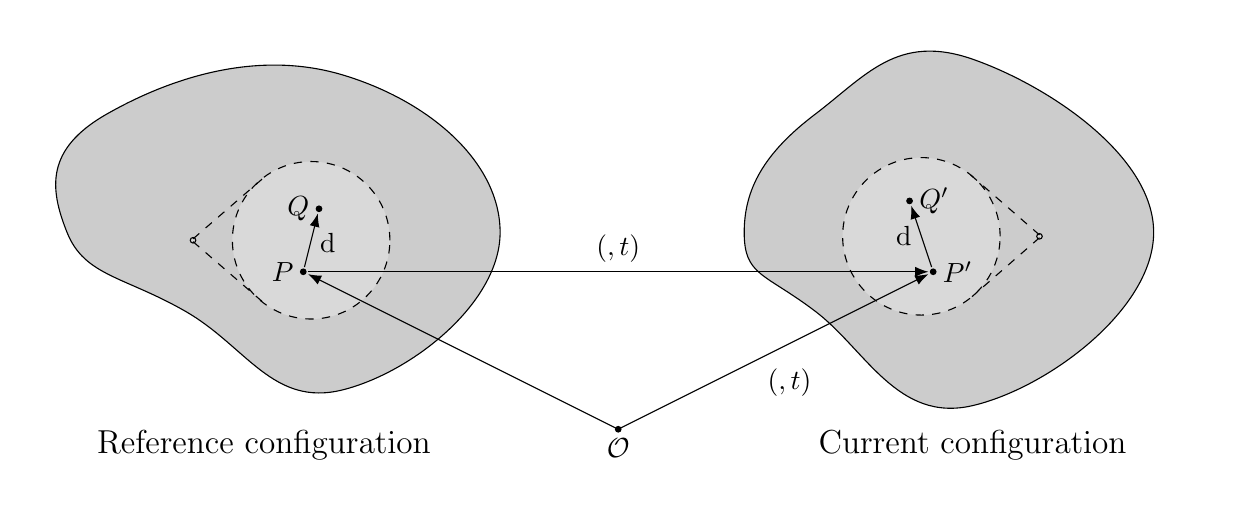
\begin{tikzpicture}[>=Latex]
    \path(-7.5,-0.8) rectangle (7.5,5.1);
    \node[inner sep=1.5] (P) at (-4,2){}; 
    \node[inner sep=1.5] (Q) at ($(P)+(0.2,0.8)$){}; 
    \node[inner sep=1.5] (PP) at (4,2){}; 
    \node[inner sep=1.5] (QQ) at ($(PP)+(-0.3,0.9)$){}; 
    \node at (-4.5,-0.2){\large Reference configuration};
    \node at (4.5,-0.2){\large Current configuration};
    \coordinate (O) at (0,0){};

    % Bodies
      \draw[fill=gray1] plot[smooth cycle, tension=0.8,shift={(-3.5,2.5)}] coordinates {(2,0)(0,2)(-3,1.5)(-3.5,0)(-2,-1)(0,-2)};
      \draw[fill=gray1] plot[smooth cycle, tension=0.8,shift={(4.5,2.5)}] coordinates {(2.3,0)(0,2.2)(-2,1.5)(-2.9,0)(-2,-1)(0,-2.2)};

    % Circles
      \draw[dashed,fill=gray2] ($(P)!0.5!(Q)$) coordinate (c1) circle (1);
      \draw[fill=gray2] ($(c1)+(-1.5,0)$) coordinate (c2) circle (1pt);
      \draw[dashed,fill=gray2] ($(PP)!0.5!(QQ)$) coordinate (c3) circle (1);
      \draw[fill=gray2] ($(c3)+(1.5,0)$) coordinate (c4) circle (1pt);

    % Points
      \draw[fill] (O) circle (1pt) node[below]{$\mathcal{O}$};
      \draw[fill] (P) circle (1pt) node[left] {$P$}; 
      \draw[fill] (Q) circle (1pt) node[left] {$Q$};  
      \draw[fill] (PP) circle (1pt) node[right] {$P'$}; 
      \draw[fill] (QQ) circle (1pt) node[right] {$Q'$}; 
      
    % Arrows 
      \draw[->] (O)--(P) node[pos=0.45,below left] {$\XX$};
      \draw[->] (P)--(Q) node[pos=0.45,right] {$\rmd\XX$};
      \draw[->] (P)--(PP) node[pos=0.5,above] {$\uu(\XX,t)$}; 
      \draw[->] (PP)--(QQ) node[pos=0.5,left] {$\rmd\xx$}; 
      \draw[->] (O)--(PP) node[pos=0.45,below right] {$\xx(\XX,t)$};

    % Lines
      \draw[dashed]($(c2)+(0,-0.5pt)$) -- ($(c1)+(235:1)$);  
      \draw[dashed]($(c2)+(0,0.5pt)$) -- ($(c1)+(125:1)$);  
      \draw[dashed]($(c4)+(0,0.5pt)$) -- ($(c3)+(52:1)$);  
      \draw[dashed]($(c4)+(0,-0.5pt)$) -- ($(c3)+(310:1)$);

  \end{tikzpicture}
\end{document}

% ,shift={(-4,2)} 